\fancychapter{Background}

In this section, we will start by generally describing what clustering is and how it works. We will then outline how ~\ac{SOM}~\cite{Kohonen1990} perform, which is the document clustering algorithm used on this thesis.

\section{Document Clustering}
\label{sec:clustering}
Document clustering is an optimal division of documents into categories without prior knowledge of the data that is being organized, based only on the similarity between them. Due to the fact that no prior knowledge of the data has to be known, document clustering is labeled as Unsupervised \ac{ML}~\cite{hinton1999unsupervised}.

~\citet{Liu2012b} asserted that document clustering can be used in a variety of Computer Science fields, such as:
\begin{itemize}
  \item Natural Language Preprocessing.
  \item Automatic Summarization.
  \item User preference mining.
  \item Improving text classification results.
\end{itemize}

There are two main types of document clustering: hard clustering and soft clustering. In hard clustering, one document can only belong to one cluster, while in soft clustering one document can belong to multiple clusters. 

%REMOVEDBYPAVEL
%In regard to document categorization~\citet{Springorum1998} performed clustering with SOMs~\citep{Kohonen1990} while identifying polysemous German Propositions. They used regular SOMs to create multiple clusters and used Centroid-Based or Preposition-based softening to create Soft Clusters from the Hard Clusters.

The clustering process usually works as described in Figure~\ref{fig:1_Text_Clustering_Main_Framwork}. In the first step, a data set must be provided with the documents to be clustered. The second step is where non relevant words are removed from the documents, to improve clustering quality~\cite{Kang2003}. 

\begin{figure}
  \begin{center}
    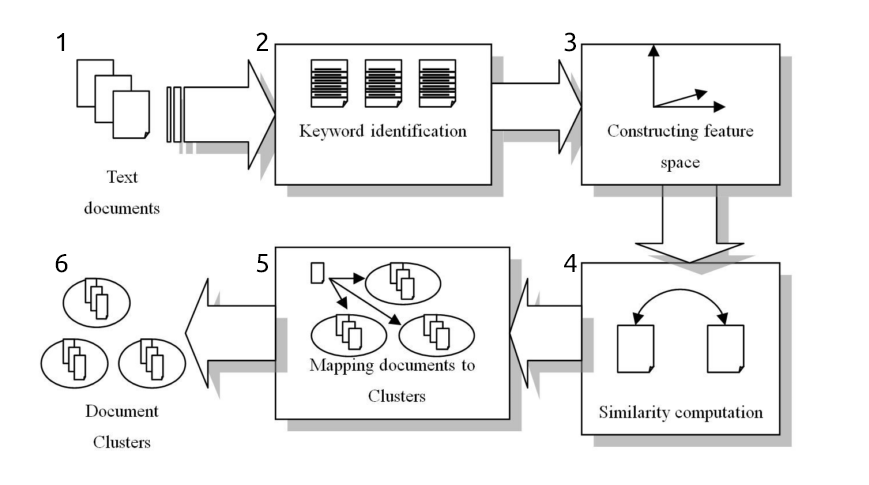
\includegraphics[width=12cm]{images/1_Text_Clustering_Main_Framwork.png}
  \end{center}
  \caption{ Text clustering main framework~\cite{Dozono2012} }
  \label{fig:1_Text_Clustering_Main_Framwork}
\end{figure}

%REMOVEDBYPAVEL
%Another way to extract keywords is to differentiate text features by analyzing the document corpora. For example if the dataset is composed from HTML or XML documents it is possible to identify more relevant features due to the characteristics of the document syntaxe.
The third step is characterized by converting the keywords of each document into vectors. The most common model used for this task is \ac{VSM}. In \ac{VSM}, each vector dimension represents one detected keyword and each document is represented by the vector of keywords in the feature space. This process is illustrated in Figure~\ref{fig:2_svm} and works in the following way:
\begin{itemize}
  \item \textbf{First step:} string tokenization, and token selection. In this case, stop words and repeated words will be removed.
  \item \textbf{Second step:} string to \ac{VSM} conversion. Each different word will correspond to a position in the array, and its value will correspond to the number of occurrences. 
\end{itemize}

\begin{figure}
  \begin{center}
    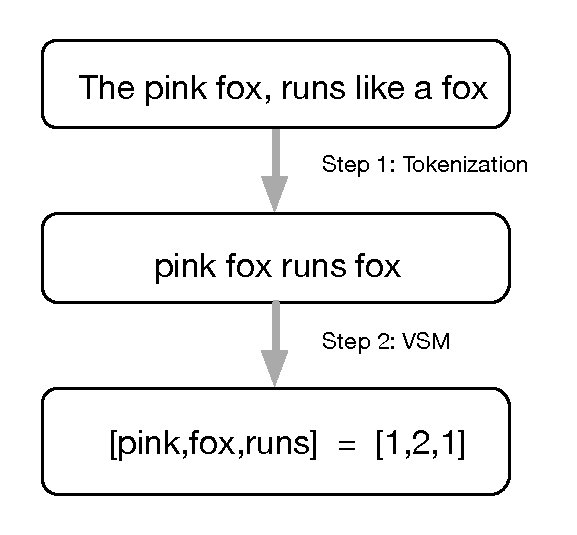
\includegraphics[width=5cm]{images/2_svm.eps}
  \end{center}
  \caption{ Text tokenization and transformation to Vector Space Model. }
  \label{fig:2_svm}
\end{figure}

There are many clustering algorithms. In the following section we will describe the particullar case of the \ac{SOM} algorithm, the solution used in our work.

\section{The Self-Organizing Map} 
\label{sec:the_self_organizing_map}

\ac{SOM} are a two layer recurrent \ac{ANN} that has the desired property of topology preservation, thus mimicking the way the cortex of highly developed animals brains work. \ac{SOM} allow cluster visualization of multi-dimensional data, similar to methods such as \ac{MDS}~\cite{KruskalWish1978} and \ac{PCA}~\cite{Hotelling_1933} .  

\citet{Bacao2005} described the basic idea behind \ac{SOM} as a mapping between input data patterns into a n-dimensional grid of neurons, or units. That grid is also know as the output space, as opposed to the initial space --- input space --- where the input patterns reside. An illustration of both spaces can be seen in Figure~\ref{fig:5_neighbours_converge}.

SOMs work in a similar way as is thought the human brain works. Analogously to the human brain, SOMs also have a set of neurons that, through learning experience, specialize in the identification of certain types of patterns. These neurons are responsible for categorizing the input patterns for which they are responsible to identify. Nearby neurons will be organized by similarity, which will cause similar patterns to activate similar areas of the \ac{SOM}.
With this topology preserving mapping, the \ac{SOM} organizes information spatially, where similar concepts are mapped to adjacent areas. The topology is preserved in a sense that, as far as possible, neighborhoods are preserved throughout the mapping process.
Output neurons are displayed in an N dimensional grid, generally rectangular, but other structures are possible, such as hexagonal or octagonal.  The grid of neurons, in the output space, can be divided in neighborhoods --- where neurons responsible for the same kind of input reside.
In \ac{SOM}, neurons will have the same amount of coefficients as the input patterns and can be represented as vectors.

Before describing the algorithm, it is important to define two key aspects of the \ac{SOM}: the learning rate and the quantization error. The learning rate is a function that will be decreased to converge to zero. It will be applied to winning neurons and their neighbors in order for them to move toward the corresponding input pattern in progressively smaller steps. Quantization error is the distance between a given input pattern and the associated winning neuron. It describes how well neurons represent the input pattern. The radius of the neighborhood around the winning neuron is also particularly relevant to the topology of the \ac{SOM}, deeply affecting the unfolding of the output space as stated by~\citet{Bacao2005}. 

In order to know how well a neuron maps to all the input patterns it represents, the average of the quantization error can be used(Eq. \ref{eq:avg_quant_error}). On the equation, $d_{i,n}$ is an input pattern that is represented by the neuron $w$. Each neuron represents an arbitrary number --$n$--of input patterns, that group of input patterns is represented as $D_{i,j}$.
\par
\begin{equation}
  \label{eq:avg_quant_error}
  \varepsilon(w) = \frac{\sum_{i=0}^{n} \| w - d_{i}  \| }{n}, d_{i} \in D, \forall n
\end{equation} 


% Self Organizing Map algorithm in latex, needs package algorithm2e
\begin{figure}[h]
  \begin{algorithm}[H]
    \label{alg:som}
    \DontPrintSemicolon
    \KwData{Input patterns $X = \{  \overrightarrow{x_1}$,\dots,$\overrightarrow{x_N}$ \}, number of iterations $t_{\textrm{$max$}}$,  neighborhood function $\sigma(t)$, learning rate  $\epsilon(t)$ }
    \KwResult{Trainned map and clustered input patterns}
    Randomly initialize neurons, $w_i \in \mathbb{R}^{D}, \forall i $ \;
    \For{ $t = 1 \; to \; t_{\textrm{$max$}}$ }{
      Randomly draw an input pattern, $ \overrightarrow{x_d} $  \;
      \nl\label{som:one}$p =  \arg{ min_i \{ \|  \overrightarrow{x_d} - \overrightarrow{w_i} \|  \}}  $  \;
      \nl\label{som:two}$\overrightarrow{w_i} = \overrightarrow{w_i} + \epsilon(t) \cdot h_{ip}(t) \cdot ( \overrightarrow{x_d} - \overrightarrow{w_i} ),  \forall{i}$ \;
      \nl\label{som:three}$\sigma(t) = \sigma_0( \sigma_f / \sigma_0 )^{t/t_{max}}$  \;
      \nl\label{som:four}$\epsilon(t) = \epsilon_0( \epsilon_f / \epsilon_0 )^{t/t_{max}}$ \;  
      \nl\label{som:fifth}$ t \leftarrow t + 1$}
      \caption{Self-Organizing Map \cite[]{Kohonen1990} }
  \end{algorithm}
\end{figure}

The learning phase is characterized by the Algorithm~\ref{alg:som}, which works the following way:
\begin{itemize}
  \item \textbf{Line 1:} The neuron closer to the input pattern is selected. The Euclidean distance (Eq.~\ref{eq:eucl_dist}) is generally used.
    \begin{equation}
  \label{eq:eucl_dist}
  Dist=\sqrt{\sum_{i=0}^{i=n}( V_i-W_i)^2}
\end{equation} 

  \item \textbf{Line~\ref{som:two}:} the winning neuron $(p)$ previously selected on line 1 is updated, in order to better represent the input pattern --- this process is represented on Figure~\ref{fig:4_wining_neuron_converge}. Also, all other neurons inside a specific radius will also be updated --- this process is described in Figure~\ref{fig:5_neighbours_converge}. Each neuron is updated with a different rate of influence determined by how far away it is from the winning neuron, which is defined by the neighborhood influence function $h_ip(t)$. A Gaussian (Eq.~\ref{eq:gaussian}) is often used. 
    \begin{equation}
  \label{eq:gaussian}
  h_{ip}(t)=\exp{-\frac{|\overrightarrow{a_i}-\overrightarrow{a_p}|^2}{\sigma^2(t)}}
\end{equation} 

  \item \textbf{Line~\ref{som:three}:} the size of the radius is updated.
  \item \textbf{Line~\ref{som:four}:} the learning rate is updated.
  \item \textbf{Line~\ref{som:fifth}:} the number of iterations is incremented.
\end{itemize}
 
In order for the algorithm to converge, the learning rate and the radius of the neighborhood need to decrease at a given rate. This process can be seen on line \ref{som:three} and \ref{som:four}, respectively .
%Generally exponential decay is used.


%TODO: Umatrix algorithm
\begin{algorithm}[H]
  \label{alg:umatrix}
  \DontPrintSemicolon
  \KwData{Input patterns $X = \{  \overrightarrow{x_1}$,\dots,$\overrightarrow{x_N}$ \}, Trainned neurons $W = \{  \overrightarrow{w_1}$,\dots,$\overrightarrow{w_N}$ \} }
  \KwResult{U-Matrix}
  \For{ $t = 1 \; to \; N$ }{
    Randomly draw an input pattern, $ \overrightarrow{x_d} $  \;
    $p =  \arg{ min_i \{ \|  \overrightarrow{x_d} - \overrightarrow{w_i} \|  \}}  $  \;
    $\overrightarrow{w_i} = \overrightarrow{w_i} + \epsilon(t) \cdot h_ip(t) \cdot ( \overrightarrow{x_d} - \overrightarrow{w_i} ),  \forall{i}$ \;
    $\sigma(t) = \sigma_0( \sigma_f / \sigma_0 )^{t/t_{max}}$  \;
    $\epsilon(t) = \epsilon_0( \epsilon_f / \epsilon_0 )^{t/t_{max}}$ \;}  
  \caption{U-Matrix }
\end{algorithm}


\begin{figure}
  \begin{center}
    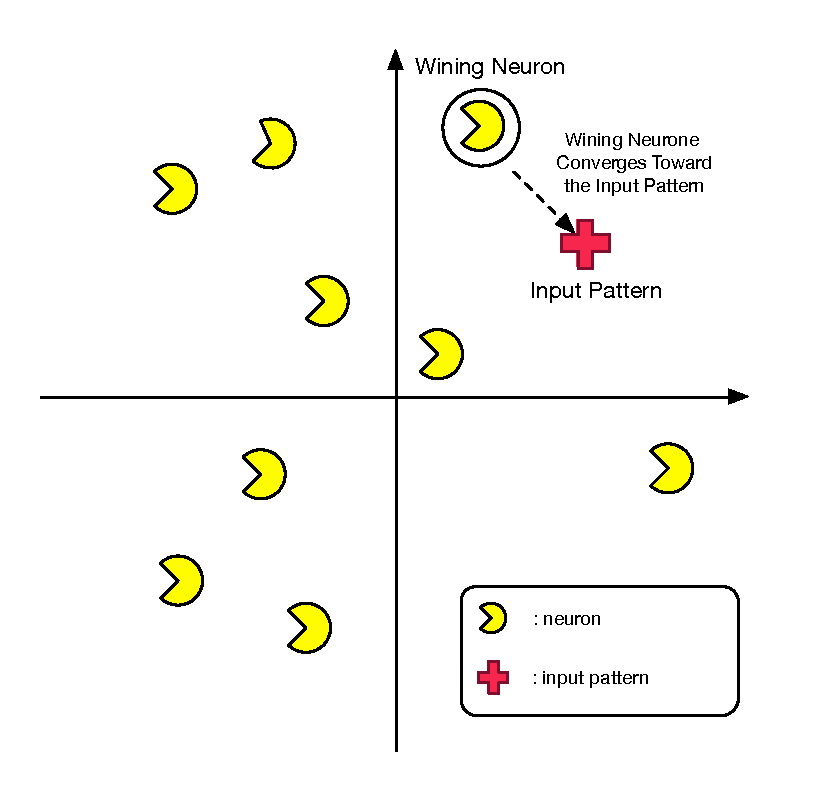
\includegraphics[width=5cm]{images/4_wining_neuron_converge.eps}
  \end{center}
  \caption{ Winning neuron converging at learning rate }
  \label{fig:4_wining_neuron_converge}
\end{figure}

\begin{figure}
  \begin{center}
    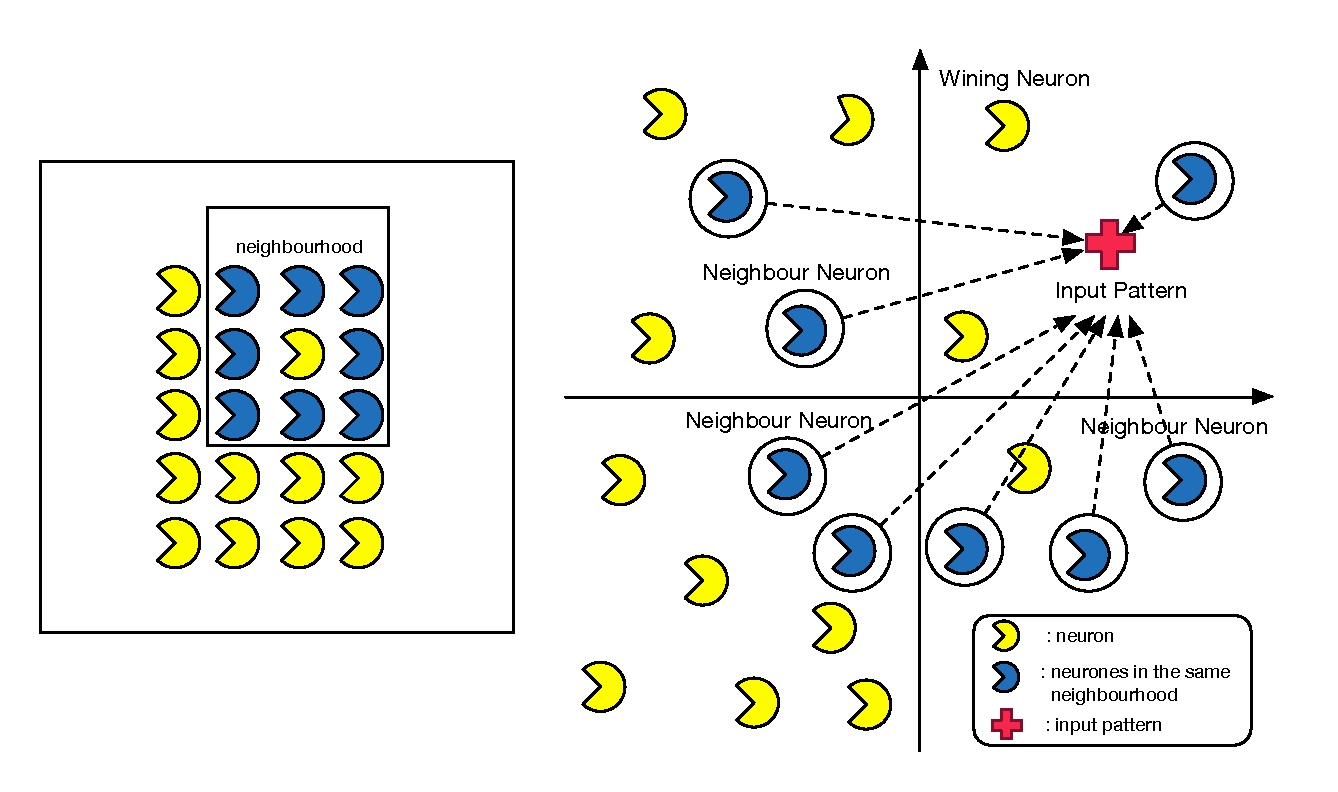
\includegraphics[width=12cm]{images/5_neighbours_converge.eps}
  \end{center}
  \caption{ On the left the output space neighborhood, on the right the neighbors of the winning neuron converging in the direction of the input pattern }
  \label{fig:5_neighbours_converge}
\end{figure}

The prediction phase can start after the model is learned. On the prediction phase, new input patterns can be quickly assigned to the \ac{SOM}, without need to apply the learning rate to the winning neuron and his neighbors. Due to the fact that the input pattern will be assigned to the cluster that is mapped by the nearest neuron. Thus, it is very easy and fast to classify new data now. As stated by ~\citet{Liu2012b}, the advantages of using \ac{SOM} are: data noise immunity, easy to visualize data, and parallel processing.

In order to visually interpret the result of the \ac{SOM}, \ac{U-Matrix} method may be used~\citep{Bacao2005}. The \ac{U-Matrix} is a representation of the \ac{SOM}, in which, the average topological error between a neuron and all the input patterns he represents is displayed in a color scale proportional to the maximum and minimum values obtained in the \ac{SOM}. 

Computing a U-Matrix is done by the Algorithm~\ref{alg:umatrix}. Essentially, each neuron is responsible for representing a cluster of input patterns. The better a neuron represents an input patter and the smaller the distance between them both. Therefor, the better a neuron represents a group of input patterns, the smaller the average distance between himself and all the input patterns it represents. 
For representation purposes, after all the averages are computed a lighter color is assigned to the lower average, and the darkest color to the highest. Thus, all the values in between must have a color proportional to its own value, in reference to the edge values. An example of an \ac{U-Matrix} can be seen in Figure~\ref{chp3:img2}.

\begin{figure}[htpb]
  \centering
  \subfigure[SOM ouputspace trained with random RGB vectors]{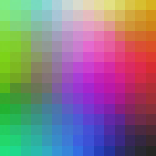
\includegraphics[scale=2]{./images/som.pdf}\label{chp3:img1}}
  \hspace*{0.5cm}
  \subfigure[U-Matrix representing how well each neuron maps to input patterns it represents]{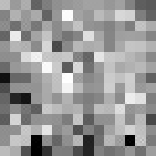
\includegraphics[scale=2]{./images/umatrix.pdf}\label{chp3:img2}}\\
  \caption{U-Matrix and SOM output space, computed by training the SOM during 400 epochs, with 1500 random input patterns representing an RGB color.}
  \label{fig:umatrix_and_ouputspace}
\end{figure}

\subsection{Quantization Error} 
\label{sub:quantization_error}
SOM training is always subject to some variability due to multiple causes, like the sensitivity of initial conditions, convergence to local minima and sampling variability, as stated by~\citet{Bodt}. This subsection will present statistical tools to measure the quality of the SOM, by measuring its quantization error. 

%and topology preservation.

The SOM Quantization Error is the mean of all Euclidean distances between the observed data points and their corresponding winning neuron. This value might vary depending on the initialization neurons or the order of the input data fed into the SOM while the training is occurring. When applied to an individual input data, represents how well a neuron is representing input data. Since the SOM Quantization Error represents the mean of all quantization errors from all the input data, generally, the lower the error is the best the SOM was trained.
\\
No general formula exists to minimize quantization error~\cite{Bodt} . What is generally done is just to change the number and values of the starting neurons and the order of the input data in order to train multiple SOMs. In the end the SOM with the lowest quantization error is chosen.
In this project since multiple approaches to the SOM algorithm and data representation will be tested, as described in Section~\ref{ssub:default_som_approach_},and the ones having the lower quantization error will be selected for the prototype.

